关于执行模型,需要了解多少?近年来,并行内核作为一种表达数据并行性的方式出现。基于内核的方法主要为了跨各种设备的可移植性,以便提高开发者工作效率。因此,内核通常不是硬编码处理特定数量或配置硬件资源(例如:内核、硬件线程、SIMD[单指令多数据]指令)。相反,内核用抽象的概念来描述并行性,实现(即编译器和运行时的组合)可以映射到特定目标设备上的可用硬件并行。尽管这种映射是由具体实现定义,但我们相信其会选择一种合理,且能够有效利用硬件并行性的映射。\par

以一种硬件无关的方式运行大量的并行计算,确保了程序可以扩展(或缩小)以适应不同平台的能力,但是……\par

\begin{tcolorbox}[colback=red!5!white,colframe=red!75!black]
保证功能的可移植性,但不保证高性能!
\end{tcolorbox}

支持的设备很多,不同的架构为不同的用例设计和优化。想要在特定的设备上达到最高的性能水平,总是需要一些手动优化工作——不管使用什么编程语言!这种特定于设备的优化的例子包括针对缓存的阻塞、选择平摊调度开销的粒度大小、使用专门的指令或硬件单元,以及选择适当的算法。其中一些例子将在第15、16和17章中继续讨论。\par

应用程序开发过程中,在性能、可移植性和生产率之间的平衡是必须面对的挑战,也是本书不能完全解决的挑战。然而,我们希望证明DPC++提供了一种高级编程语言,还提供了可维护通用可移植代码和优化目标特定代码所需的所有工具。\par

\hspace*{\fill} \par %插入空行
\textbf{多维内核}

许多语言的并行构造是1维的,直接将工作映射到1维硬件资源(例如:硬件线程数)。并行内核是一个更高层次的概念,维度更多地反映了代码要解决的问题(在1、2或3维空间中)。\par

为了在1维空间开发方便,并行内核提供的多维索引。理解这个映射的行为方式可能是某些优化(例如:调优内存访问模式)的重要部分。\par

需要思考的是,哪个维度是连续的或“单位跨距”(即,多维空间中的数据落在一维空间中的位置)。SYCL中与并行性相关的多维变量都遵循相同的约定:维度从0到N-1进行编号。这种约定与标准C++中多维数组的行为一致。\par

SYCL将二维空间映射为线性索引的示例如图4-1所示。也可以打破这种方式,采用自己的方法来线性化索引,这样做必须小心——打破惯例可能会对让步长为1访问方式有性能收益的设备产生负面的性能影响。\par

\hspace*{\fill} \par %插入空行
图4-1 映射二维范围(2,8)到线性索引上
\begin{center}
	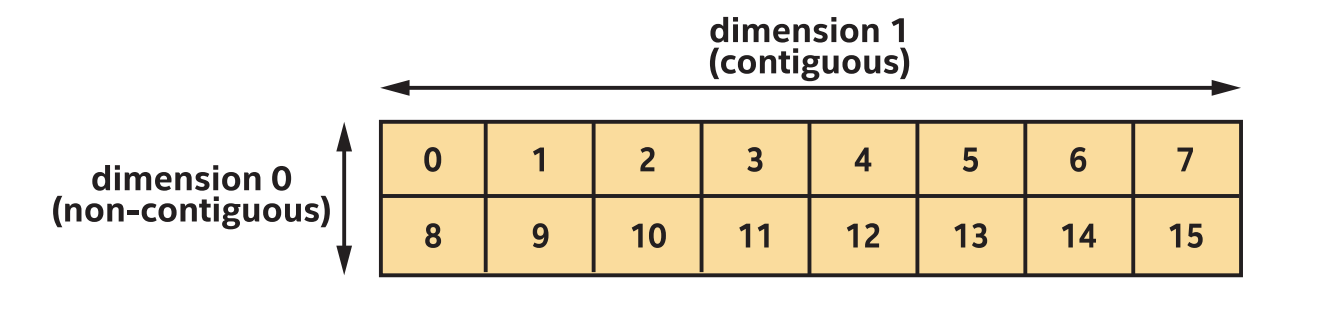
\includegraphics[width=1.\textwidth]{content/chapter-4/images/2}
\end{center}

如果程序数据大于三个维度,则必须使用模算法手动负责多维索引和线性索引之间的映射。\par

\hspace*{\fill} \par %插入空行
\textbf{循环与内核}

迭代循环是一种串行结构:循环的每次迭代都按顺序执行。优化的编译器可以确定迭代循环的部分或全部是否可以并行执行,但必须是保证,当编译器无法证明并行执行是安全的,则保持循环顺序语义的正确性。\par

\hspace*{\fill} \par %插入空行
图4-2 用串行循环表示向量加法
\begin{lstlisting}[caption={}]
for (int i = 0; i < N; ++i) {
	c[i] = a[i] + b[i];
}
\end{lstlisting}

考虑图4-2中的循环,描述了简单的向量加法。即使在这样的情况下,证明循环可以并行执行也不是一件简单的事情:只有当c不重叠a或b时,并行执行才安全。而在一般情况下,没有运行时检查是无法证明这一点的!为了解决这样的情况,语言添加了一些特性,使我们能够向编译器提供信息,从而简化分析(例如,断言指针不与restrict重叠)或完全覆盖所有情况进行分析(例如,声明循环的所有迭代都是独立的,或者确切地定义应该如何将循环调度为并行资源)。\par

并行循环的含义有些含糊不清——因为不同的并行编程语言会重载这个术语——但是许多常见的并行循环构造表示,编译器转换顺序循环。这样的编程模型使我们能够编写顺序循环,并且只需要提供有关如何安全地并行执行不同迭代的信息。这些模型非常强大,与其他编译器优化集成得很好,并且极大地简化了并行编程,但这不代表鼓励开发者在开发的早期阶段考虑并行性。\par

并行内核不是循环,也没有迭代。相反,内核表示一个操作,可以多次实例化,并应用于不同的输入数据;当内核并行启动时,该操作的多个实例将同时执行。\par

\hspace*{\fill} \par %插入空行
图4-3 将循环重写(伪代码)为并行内核代码
\begin{lstlisting}[caption={}]
launch N kernel instances {
	int id = get_instance_id(); // unique identifier in [0, N)
	c[id] = a[id] + b[id];
}
\end{lstlisting}

图4-3展示了使用伪代码重写为内核的简单循环示例。这个内核中实现并行性是明确的:内核可以由任意数量的实例并行执行,每个实例独立地应用于单独的数据块。通过将此操作编写为内核,可以确定并行运行是安全的(理想情况下应该如此)。\par

简而言之,基于内核的编程不是一种使用并行改进顺序代码的方法,而是一种编写显式并行程序的方法。\par

\begin{tcolorbox}[colback=red!5!white,colframe=red!75!black]
我们越早将思路从并行循环转向内核,就越容易使用Data Parallel C++编写高效的并行程序。
\end{tcolorbox}
























